\chapter{La remise en conformité du Sondeur de canal}

Le sondeur de canal est réalisé par mon tuteur M Jean-pierre BARBOT en 1995 dans le cadre du projet CNET RAMEAU. Ce sondeur de canal a pour fonction de caractériser le canal de propagation afin de fournir des études de cas,des statistiques et des modélisation du canal. Ceci est utilisé lors de la dimensionnement de la puissance de la station de base et des équipement mobile. A l'époque où les sondeurs de canal ont une dimension immense échelle d'un camion, ils ont crée un sondeur de dimension 1,5m*0.8m*0.8m. Ce qui leur permet de réaliser des essais à l'intérieur des bâtiment. Ceci a pour but de couvrir les réseau mobile à l'intérieur des bâtiments.Ensuite le sondeur a été modifié pour un autre projet après quelques années, les modifications apportés a causé des soucis. Une partie de la commande d'acquisition est endommagée.  \\

Dans la première partie nous nous intéressons tout d'abord à analyser les effets perturbateurs subis par le signal dans le canal de propagation et sa modélisation choisie. Ainsi que l'identification des matérielles constituées par le sondeur. Par la suite commence les essais sur le sondeur pour identifier si une autre partie est tombé en panne. Pour conclure l'objectif final de cette partie consiste à remplacer les composants hors-service, de mettre à jour les composants qui sont obsolètes et également d'optimiser l'espace utilisée pour réduire la taille du sondeur. Pour ce faire il faut tout d'abord optimiser l'espace vide entre les composants, puis il faut voir s'il est intéressant de remplacer les composants encombrants par celles qui ont la même fonctionnalité mais occupe moins d'espace. Dans de remettre le sondeur en état de marché.

\section{Caractérisation du canal de propagation}

Nous souhaitons établir une radiocommunication entre une base et mobile dans la bande de U.H.F.      \ (1-3 GHz). Il y a une fluctuation entre le signal reçus et émis, ceci est dû aux différents effets de perturbation introduits par le canal de propagation. Ces effets sont détaillés dans la suite de la section "Effets du canal de propagation".\\ 
\newpage
\subsection{Canal de propagation}

Le canal de propagation est le lien physique entre l'émetteur et le récepteur des signaux.  Les éléments situés dans le canal de propagation réduisent l'amplitude du signal, en cause ces éléments ont un indice de radio-opacité qui réduit la puissance du signal. La zone de propagation du signal dépend de l'angle d'émission de l'antenne émettrice. L'antenne réceptrice peut recevoir des différentes versions du signal qui a un délai ou déphasé par rapport au signal initialement émis. En effet lorsque les ondes entrent en contact avec des objets réfléchissants dans le canal,ils sont dérivés et changés de direction de propagation. Par conséquent les ondes ne sont pas initialement orientées dans la direction de l'antenne réceptrice vont finalement atteindre cette antenne. On appelle ce phénomène propagation multi-trajet. Les chemins de parcours des ondes sont illustrés sur la figure suivante.\\
\fig{1}{trajetm.png}{Phénomène du trajet multiple}

%bibliohttp://https://www.slideshare.net/ShreeKrupa1/multichannel-fading

\begin{itemize}[label=\ding{93}, font=\large \color{lightgray}]
\item La réflexion : lorsque l'onde électromagnétique du signal rencontre dans sa direction une surface lisse dont les dimensions sont grandes par rapport à la longueur d'onde du signal.

\item La diffusion : lorsque l'onde électromagnétique du signal entre en collision avec une surface dont la surface n'est pas parfaitement plane et lisse. Ce phénomène engendre la diffusion de l'onde dans plusieurs directions.

\item La diffraction : lorsque l'onde électromagnétique heurte une arête d'un corps volumineux dont les dimensions sont grandes (les bâtiments, les collines) par rapport à la longueur d'onde  du signal. Le signal contourne l'obstacle et continuer à se propager derrière celui-ci accompagnée d'une atténuation de la puissance.\\
\end{itemize}

C'est pour cette raison que les signaux reçus par les antennes peut être issue de ces deux chemins différent:\\
\begin{enumerate}
\item Le signal direct (Line of sight en anglais) : c'est le signal qui a parcouru le chemin de propagation le plus court. 
\item Le signal indirect (No Line of sight en anglais) : le signal qui a été réfléchit,diffracté ou diffusé par un élément dans le canal de propagation. Il existe une atténuation de la puissance et une latence entre le moment de la réception du signal direct et ce signal,en raison de chemin de propagation plus longue.\\
\end {enumerate} 

Dans la plupart des cas le signal indirect est considéré comme une interférence qui perturbe la reconstruction du signal émis. Dans le cas où le signal indirect a une déphasage d'un multiple d'une demi-période par rapport au signal émis,le signal reçus est fortement atténué par celui-ci. Dans le cas où le signal indirect a une déphasage d'un multiple d'une période, le signal est amplifié. Et dans le cas où un obstacle de grande est sur le chemin direct et atténue fortement ou masque complètement le signal. Le signal indirect devient très utile pour reconstruire le signal émis.


\subsection{Effets introduits par le canal de propagation}
\label{Effets}

Lors de la réception des signaux, on constate qu'il y a une recombinaison des signaux directs et indirects. Le signal reçus subit des phénomènes de perturbation qu'on peut catégoriser par la variabilité spatiale et la sélectivité fréquentielle.

\subsubsection{Variabilité spatiale}

La variabilité spatiale a pour effet d'atténuation de la puissance du signal reçus et d'introduire des erreurs. On catégorise cet effet en 3 échelles de fluctuation.\\
\begin{enumerate}
\item Les évanouissements rapides qui sont l'origine des paquets d'erreurs introduisent lors d'une communication numérique. Dans le cas de la communication analogique ils sont la cause de la modulation de fréquence aléatoire qui perturbe le système.

\item Une affaiblissement dite moyenne échelle. La cause d'influence est l'environnement du canal de propagation. Les bâtiments situés dans le canal produisent un effet de masque qui atténue le signal. La météo peut également avoir un impact. Lors que 

\item Une affaiblissement dite grande échelle est dû essentiellement aux déplacement du récepteur mobile, l'amplitude du signal change en fonction de la distance sépare de l'émetteur et le récepteur.

\end{enumerate}
\subsubsection{Sélectivité fréquentielle}

La sélectivité fréquentielle que manifeste le canal est dû également au trajet multiple du signal. Un très grand débit impose une grande bande passante et si cette bande passante "couvre" une partie du spectre comportant des creux (dus aux trajets multiples), il y a perte totale de l'information pour la fréquence correspondante. Lorsque le débit de transmission est élevé les signaux indirects reçus vont gêner la reconstitution du signal émis lors de la réception des signaux par l'antenne. En conséquence pour que le signal soit bien transmis il faut que la durée des symboles (c'est-à-dire le temps qui sépare 2 séquences de N données) adapte à la dispersion des retards. C'est l'écart-type de la fonction densité de puissance($P_h$), elle est exprimé par:\\
\[ P_h(0,\tau)=\lim_{t->\infty}(\frac{1}{T}\int_{\frac{T}{2}}^{-\frac{T}{2}}h(t_2,\tau)h^{*}(t_2,\tau)dt_2) \]

 Ce qui vas limiter le débit maximum. Sur la figure suivante on constate une partie du signal initial émis est recouvert par les signaux indirects et déphasés et ainsi la reconstruction du signal de base peut ne pas être réalisable.
%\fig{0.85}{écho.png}{Phénomène du trajet multiple}
\\
\subsection{Mesure du canal de propagation}

La fonction principale du sondeur est de caractériser le canal. Dans cette partie nous allons voir le modèle choisi du canal et comment isoler pour obtenir la caractérisation du canal.

\subsubsection{Modèle du canal de propagation}	
 
Nous souhaitons mettre les effets introduits dans le canal sous équation. La modélisation choisi est issue de la modélisation dite boite noire. \\
\begin{center}
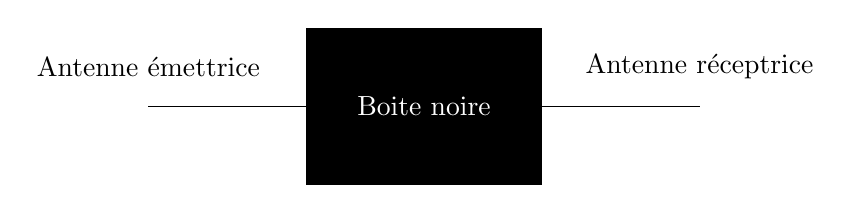
\begin{tikzpicture}
\node at (0,1.5) {Antenne émettrice};
\draw (0,1)--(2,1);
\fill[black] (2,0) -- (2,2) -- (5,2) -- (5,0);
\node at (3.5,1)[white] {Boite noire};
\draw (5,1)--(7,1);
\node at (7,1.5) {Antenne réceptrice};
\end{tikzpicture}
\end{center}
L'étude des équations de Maxwell réagissant aux effets montre que ces effets induits dans les différents version du signal est linéaire. Dans le cadre de notre mesure, le temps d'échantillonnage est relativement faible,
on suppose que les caractéristiques du canal n'évolue pas pendant le temps de mesure.Donc nous modélisons le canal en utilisant le modèle de la boite noire par un filtre linéaire invariant, sous la forme suivante : \\
\[ s(t)= \int_{+\infty}^{-\infty} I(t,\tau)*e(t- \tau)\,\mathrm{d}\tau \]
avec
\begin{itemize}[label=\ding{93}, font=\large \color{lightgray}]
\item e(t): le signal émis
\item s(t): le signal reçu
\item $I(t,\tau):$ la réponse impulsionnelle du canal à l'instant t pour une impulsion de Dirac émise à l'instant$(t-\tau).$
\end{itemize}
Sous l'enveloppement complexe s'exprime de cette façon:
\[ y(t)= \int_{+\infty}^{-\infty} h(t,\tau)*x(t- \tau)\,\mathrm{d}\tau \]
avec
\begin{itemize}[label=\ding{93}, font=\large \color{lightgray}]
\item x(t): l'enveloppe complexe du signal émis
\item y(t): l'enveloppe complexe du signal reçu
\item $h(t-\tau) \text{l'enveloppe complexe de } \frac{1}{2}I(t-\tau)$ 
\end{itemize}
Nous considérons que les effets de propagation sont aléatoire donc la modélisation est construite sous l'hypothèse de WSSUS.

\subsubsection{Méthode choisie pour réaliser la mesure}

A partir de l'équation sous l'enveloppement complexe et la propriété du produit de convolution fait que la convolution des signaux peut s'exprimer de cette manière :

\[ R_{xy}(t)= \int_{+\infty}^{-\infty} h(t,\tau)*R_{xx}(t- \tau)+R_{xb}(t) \]
 avec 
\begin{itemize}[label=\ding{93}, font=\large \color{lightgray}]
\item $ R_xy(t) $: la corrélation du signal émis avec le signal reçu
\item $ R_xx(t) $: l'auto-corrélation du signal émis
\item b(t): 	\quad le bruit contenu dans la mesure
 %\[ R_xy(t) \text{La corrélation du signal émis avec le signal reçu}\]
 %\[ R_xx(t) \text{L'autocorrélation du signal émis}\]
 %\[ b(t) \text{b est le bruit contenu dans la mesure}\]
\end{itemize}

Le cas le plus simple pour les  où Rxx(t) est une impulsion de Dirac. La convolution de Rxx(t) avec h(t) donne tout simplement h(t) en raison de la propriété neutre du Dirac face à une convolution. On sait que l'auto-corrélation du bruit blanc est une impulsion Dirac. Mais le soucis est que lors des mesures il est impossible d'utiliser un signal qui a une durée infinie et non périodique. Donc il convient d'utiliser un signal fini périodique qu'on appelle un Pseudo-bruit qui donc sa fonction d'auto-corrélation est d'un triangle pointu. 
\fig{0.3}{autoc.png}{auto-corrélation du pseudo bruit}\\
Et sa densité spectrale de puissance est la suivante, en exploitant la zone autour de 0, on peut le considéré comme la DSP d'un bruit blanc.
\fig{0.3}{dsp.png}{Densité spectrale de puissance du pseudo bruit}\\
La méthode qui permet de générer une séquence de Pseudo-bruit est donné dans la figure suivante.
\label{gene code pseudo}
\fig{0.8}{pseudo.pdf}{Génération de la suite de donnée pseudo aléatoire}\\
Une partie des suites de bouclage de la contre-rétroaction nécessitant qu'une seul opération ou exclusif avec la sortie afin d'obtenir les séquence de donnés est donné dans ce tableau:
\fig{0.5}{shifttable.jpg}{Tableau de la contre-rétroaction}\\
%label=\textbullet
\begin{itemize}[label=\ding{93}, font=\large \color{lightgray}]
\item n : le nombre de registre utilisé
\item m : le bouclage de la contre-rétraction sur ce registre
\item n-m : une autre possibilité de bouclage de registre
 %\[ R_xy(t) \text{La corrélation du signal émis avec le signal reçu}\]
 %\[ R_xx(t) \text{L'autocorrélation du signal émis}\]
 %\[ b(t) \text{b est le bruit contenu dans la mesure}\]
\end{itemize}

Pour lancer le générateur de code, il faut initialiser en mettant le registre 1 à 1.La séquence de données aléatoires vont être servi pour créer un signal rectangulaire de période $ {T_s=(2^{n}-1)T_H} $ ($ f_H$ étant la  fréquence d'horloge utilisé par l'ensemble des composant $T_H=\frac{1}{f_H}$), sur une période $T_s$ on compte $2^{n-1}$ digit $2^{n-1}-1$ digit 0. 
Le temps d'acquisition doit être impérativement le multiple de la période de répétition de la séquence pseudo-aléatoire.
%F.de COULON Théorie et traitement des signaux
%% a faire le principe de pseudo bruit


\section{Etat de l'art de la version actuelle du sondeur}

\fig{0.8}{Emetteurv2.pdf}{Version actuelle de l'émetteur}
\fig{0.70}{Recepteurv2.png}{Version actuelle de du récepteur}